%----------------------------------------------------------------------------------------
%	THESIS
%----------------------------------------------------------------------------------------

\author{Panu Leppäniemi}
\title{Automaattinen keskustelun visualisointi}

\def\metropoliadegree {insinööri (AMK)}
\def\metropoliadegreeprogramme {tietotekniikka}
\def\metropoliaspecialisation {ohjelmistotekniikka}
\def\metropoliainstructors {
lehtori Olli Hämäläinen\newline
professori Olli Alm
}
\def\metropoliakeywords {keskustelun yhteenveto, visualisointi, analysointi}

%----------------------------------------------------------------------------------------
%	GLOBAL STYLES
%----------------------------------------------------------------------------------------

\documentclass[11pt,a4paper,oneside]{memoir}
\usepackage[latin1]{inputenc}
\usepackage[T1]{fontenc}
\usepackage[finnish]{babel} %change this depending on your language
\usepackage{amsmath}
\usepackage{amsfonts}
\usepackage{amssymb}
\usepackage{fontspec}
\usepackage{tocloft}
\usepackage{lipsum}
\usepackage{titlesec}
\usepackage{url}
\usepackage{mathtools}
\usepackage{float}

%condition for adding or not space in TOC
\usepackage{etoolbox}
%for compact list
\usepackage{enumitem}
%for block comment
\usepackage{verbatim}
%for "easier" references
\usepackage{varioref}
%forcing single line spacing in bibliography
\DisemulatePackage{setspace}
\usepackage{setspace}
%including figure (image)
\usepackage{graphicx}
%change the numbering for figure
\usepackage{chngcntr}
%strike trough
\usepackage{ulem}
%euro symbol
\usepackage{eurosym}

%NORMAL TEXT
%all text, title, etc. in the same font: Tahoma
\setmainfont{Tahoma}
%line space
\linespread{1.5}
%\doublespacing
%margin
\usepackage[top=2.5cm, bottom=3cm, left=4cm, right=2cm, nofoot]{geometry}
\setlength{\parindent}{0pt} %first line of paragraph not indented
\setlength{\parskip}{16.5pt} %one empty line to separate paragraph
%list with small line space separation
\tightlists

%IMAGE - FIGURE
%the figures should be placed in the "illustration" folder
\graphicspath{{illustration/}}
%figure number without chapter (1.1, 1.2, 2.1) to (1, 2, 3)
\counterwithout{figure}{chapter}
%border around images
\setlength\fboxsep{0pt}
\setlength\fboxrule{0.5pt}
%caption font size
\captionnamefont{\small}
\captiontitlefont{\small}
%space after figure caption (and other float elements)
\setlength{\belowcaptionskip}{-7pt}

%CODE
\newfloat{program}{htp}{lop}
\floatname{program}{Esimerkkikoodi}

%TOC
%remove dots
\renewcommand*{\cftdotsep}{\cftnodots}
%chapter title and page number not in bold
\renewcommand{\cftchapterfont}{}
\renewcommand{\cftchapterpagefont}{}
%sub section in toc
\setcounter{tocdepth}{2}
%subsection numbered
\setcounter{secnumdepth}{2}
\renewcommand{\tocheadstart}{\vspace*{-15pt}}
\renewcommand{\printtoctitle}[1]{\fontsize{13pt}{13pt}\bfseries #1}
\renewcommand{\aftertoctitle}{\vspace*{-22pt}\afterchaptertitle}
%spacing afer a chapter in toc
\preto\section{%
  \ifnum\value{section}=0\addtocontents{toc}{\vskip11pt}\fi
}
%spacing afer a section in toc
\renewcommand{\cftsectionaftersnumb}{\vspace*{-3pt}}
%spacing afer a subsection in toc
\renewcommand{\cftsubsectionaftersnumb}{\vspace*{-1pt}}

%TITLES
%chapter title
\titleformat{\chapter}
{\fontsize{13pt}{13pt}\bfseries\linespread{1}}
{\thechapter}{.5cm}{}
\titlespacing*{\chapter}{0pt}{.32cm}{9pt}
\titleformat{\section}
{\fontsize{12pt}{12pt}\linespread{1}}
{\thesection}{.5cm}{}
\titlespacing*{\section}{0pt}{14pt}{6pt}
\titleformat{\subsection}
{\fontsize{12pt}{12pt}\linespread{1}}
{\thesubsection}{.5cm}{}
\titlespacing*{\subsection}{0pt}{14pt}{6pt}

%QUOTE
\renewenvironment{quote}
  {\list{}{\rightmargin=0pt\leftmargin=1cm\topsep=-10pt}%
  \item\relax\fontsize{10pt}{10pt}\singlespacing}
  {\endlist}

%BIBLIOGRAPHY
%bibliography title to be "references"
\renewcommand\bibname{References}
\makeatletter %reference list option change
\renewcommand\@biblabel[1]{#1\hspace{1cm}} %from [1] to 1 with 1cm gap
\makeatother %
\setlength{\bibitemsep}{11pt}

\begin{document}
%page number always on the top right, clear the "chapter/section" head
\pagestyle{myheadings}
\markright{}
%clear chapter "title" foot page
\makeevenfoot{plain}{}{}{}
\makeoddfoot{plain}{}{}{}

%----------------------------------------------------------------------------------------
%	TITLE PAGE
%----------------------------------------------------------------------------------------

%TODO

%----------------------------------------------------------------------------------------
%	ABSTRACT
%----------------------------------------------------------------------------------------

%TODO check lineheights
%TODO add "Abstract" to the upper right corner
%TODO add Metropolia logo (check if it also exists in the Bachelor thesis)
%TODO abstract keyword section
%TODO improve padding
\pagestyle{empty}
\begin{tabular}{ | p{4,7cm} | p{10,3cm} |}
  \hline
  Authors(s) \newline
  Title \newline\newline 
  Number of Pages \newline
  Date
  & 
  Your name \newline %TODO refer to {author}
  Your title \newline\newline %TODO refer to {title}
  xx pages + x appendices \newline %TODO dynamic numbering
  \today		
  \\ \hline
  Degree & \metropoliadegree
  \\ \hline
  Degree Programme & \metropoliadegreeprogramme
  \\ \hline
  Specialisation option & \metropoliaspecialisation
  \\ \hline
  Instructor(s) & \metropoliainstructors
  \\ \hline
  \multicolumn{2}{|p{15cm}|}{
  Abstract content
  } \\[14cm] \hline
  Keywords & \metropoliakeywords
  \\ \hline
\end{tabular}
\clearpage

%----------------------------------------------------------------------------------------
%	TABLE OF CONTENTS
%----------------------------------------------------------------------------------------

\makeevenhead{plain}{}{}{}
\makeoddhead{plain}{}{}{}
\pagestyle{empty} %remove page number in toc (if longer than 2 pages)
\tableofcontents*
\pagestyle{empty} %remove page number in toc (if longer than 1 pages)
\clearpage
\pagestyle{plain}

%list of figure, tables comes here...

%abbreviation comes here...

%page number always on top right; also for chapter "title" page
\makeevenhead{plain}{}{}{\thepage}
\makeoddhead{plain}{}{}{\thepage}

\setcounter{page}{1} %page 1 should be Introduction

%----------------------------------------------------------------------------------------
%	CONTENT
%----------------------------------------------------------------------------------------

\chapter{Johdanto}
Taideprojekti.

Tavoitteena on selvittää, voiko keskustelun automaattisesta visualisoinnista ja yhteenvedosta olla hyötyä keskustelun kokonaisuuden hahmottamisen suhteen. Samalla todennetaan insinöörityössä hyödynnettävän Juju-ohjelmiston käyttökelpoisuus.

Keskustelun osalliset ja heidän väliset suhteet vaikuttavat keskustelun kulkuun ja lopputulokseen. Mielenkiinnon kohteet keskustelussa vaihtelevat osallisten kontribuutiolla \cite[s. 1]{finding-topics-in-dynamical-text}. 

Auttaako visualisointi dialektiikan eli keskinäisviestinnän todentamisessa? Puhuvatko ihmiset samoista asioista, vai ilmaisevatko he omia ajatuksiaan sivuuttaen keskustelukumppanin sanoman? Jatkuuko keskustelu rakentavasti, vai toistetaanko vanhoja teesejä etenemättä mihinkään?

Kenen aloittamista aiheista puhutaan? Kenellä on ollut valtaa ohjata keskustelun kulkua? Kuka tuo keskusteluun uutta sisältöä ja kuka toistelee aikaisemman keskustelun asettamia teemoja?

Onko keskustelun sisältö helpompi hahmottaa, kun siitä on etukäteen tehty automaattinen yhteenveto? Voidaanko nähdä keskustelusta uusia puolia, jotka on varsinkin laajoissa keskusteluissa vaikea havaita?

Automaatiossa saattaa olla myös vaaransa. Automatisoitu tulkinta karsii suuren osan keskustelun elementeistä pois. Joskus toiselle ihmisellekin on haastellista tulkita esimerkiksi sarkasmia tai ironiaa, joten vaarana on, että automatisoitu tulkinta tuottaa täysin vääriä tuloksia.

...

\chapter{Käyttötapaukset}

\section{Esivaatimukset}
Järjestelmä vaatii, että analysoitava aineisto on sähköisessä muodossa, jonka formaatti kuvaillaan taulukossa \ref{taulukko:aineistoformaatti}. Siksi toistaiseksi realististen käyttökohteiden skaalaa joudutaan rajaamaan esimerkiksi pikaviestimillä tapahtuviin tai jo valmiiksi litteroituihin keskusteluihin.

\section{Toimittajat}
Toimittajat joutuvat käsittelemään päivittäin nopeasti suurenkin määrän tietoa. Koneellinen yhteenveto voisi vähentää keskusteluiden tulkinnanvaraisuutta ja tarjota artikkelin kirjoittamista tukevia esillenostoja. Automaatiolla toimittajalla olisi mahdollista tarkastella asiaa täysin objektiivisesta näkökulmasta.

Artikkelin kirjoitettuaan toimittaja voisi verrata omaansa koneellisesti generoituun yhteenvetoon. Samalla hän voisi varmistua siitä, ettei jokin keskeisesti esillä ollut asia jäänyt häneltä vahingossa mainitsematta.

\section{Palaverit}
Esimerkiksi palavereissa, asiakastapaamisissa ja vastaavissa vähintään yhden osallistujan kannattaa ottaa sihteerin rooli. Tämä tarkoittaa sitä, että hänen mahdollisuutensa osallistua keskusteluun vähenee merkittäväksi. Varsinkin pienemmässä projektiryhmässä yhden henkilön irroittaminen kyseiseen tehtävään ei aina ole mahdollista. Tunnetusti ihminen ei ole tehokas suorittamaan useita tehtäviä samanaikaisesti [etsi järkevä lähde]. Tämä saattaa johtaa siihen, ettei palaverin aikana kirjoitetun muistion laatu vastaa aina haluttua. Ratkaisua tähän ongelmaan on pohdittu luvussa \ref{automaattinen-litterointi}.

Jos nähdään, mitä aiheita palaverin aikana on käsitelty ja samalla kerätään huomioita, mitä asioita palaverin ansiosta on päätetty, voidaan mahdollisesti useamman palaverin jälkeen alkaa muodostaa mielikuvaa siitä, käsitelläänkö samaa aihetta useissa palavereissa saamatta aikaan mitään konkreettista lopputulosta. Näin voidaan nostaa esille hankalat päätökset ja korostaa niiden käsittelyä seuraavassa tilaisuudessa.

Samalla voidaan kiinnittää huomiota erilaisiin keskustelijoihin. Yhteenvedosta voisi kartoittaa ovatko kaikki keskusteluun osalliset täysin välttämättömiä palaverin etenemisen kannalta, vai olisiko kustannustehokkaampaa pienentää palaveriin osallistuvien työntekijöiden määrää.

\section{Automaattinen litterointi - tulevaisuus\label{automaattinen-litterointi}}
Palavereista ja vastaavista tehdään usein muistiinpanot, joihin kirjataan yleensä vain pääpiirteet kiinnittämättä huomiota yksityiskohtiin. Kattavan analysoinnin kannalta tämä ei sisällä tarpeeksi dataa.

Yksi vaihtoehto riittävän tietomäärän kartuttamiseen on keskustelun äänittäminen muistiin, jolloin mikään käsitelty asia ei jäisi kirjaamatta. Ratkaisu on kuitenkin kömpelö, eikä soveltuisi varsinkaan pitkäkestoisiin keskusteluihin, koska nauhoituksen läpikäyminen ja litterointi jälkikäteen esimerkiksi yhteenvedon kirjoittamista varten veisi aikaa. Toiseksi voisi olla hankalaa hahmottaa kuka vuorollaan on ollut äänessä.

Parempi ratkaisu olisi automaattinen litterointi. Puhe muutettaisiin automaattisesti tekstimuotoon. Automaatiolla vältettäisiin manuaalisen litteroinnin virheet ja tulkinnanvaraisuudet.

Jatkuvan puheen muuttamiseksi tekstiksi on olemassa valmiita sovelluksia. Valtaosa sovellustarjonnan tekniikasta perustuu Markovin piilomalliin. Toistaiseksi rajoite teknologian yleistymiselle on ollut tulkinnan epätarkkuus \cite{lai-lu-chao:performance-analysis-of-sr-software}.
 
Puhetunnistus kuitenkin kehittyy jatkuvasti. Esimerkiksi Microsoft esitteli teknologiaansa reaaliaikaiseen puhetunnistukseen. Microsoftin omien sanojen mukaan teknologia  \textquotedblleft parantaa tulkinnan tarkkuutta huomattavasti sitten Markovin mallin lanseerauksen vuonna 1979\textquotedblright ~\cite{microsoft:breakthrough-in-speech-translation-technology}.

Valitettavasti suurin osa varsinkin suomenkielisestä sovellustarjonnasta keskittyy yksinkertaiseen puheentunnistukseen, jota voidaan hyödyntää esimerkiksi puheohjauksessa. Tällainen sovellus on tehty tunnistamaan ennaltamääriteltyjä, usein yksiosaisia komentoja. Dragon Dictation -tuoteperheen englanninkielistä palvelinpuolen sovellusta olisi voitu hyödyntää insinöörityössä, mutta tiedon eristämisen koneisto, Juju, prosessoi toistaseksi ainoastaan suomenkieltä. Näin ollen automaattinen litterointi jää toistaiseksi teoriatasolle.

Kuvitellaan kuitenkin automaattisen litteroinnin olevan mahdollista. Jotta tallenteen analysointi olisi mielekkäämpää keskustelun näkökulmasta, puheenvuoroihin pitäisi liittää identiteettitieto.

Teknisesti helpompi ja luotettavampi vaihtoehto olisi jakaa keskustelun osallisille henkilökohtaiset mikrofonit. Vastaavanlaisia ratkaisuja on ehdotettu aikaisemminkin \cite{visualizing-audio-in-group-table-conversation}. Mikrofoneihin liitettäisiin puhujan henkilöllisyys joko etu- tai jälkikäteen.

Edellämainitun ratkaisun avulla pystyisimme keräämään keskustelusta taulukossa \ref{taulu:aineistoformaatti} esitetyn formaatin mukaista dataa. Järjestelmä olettaa, että analysoitava aineisto tuodaan järjestelmään CSV-tiedostona, joka noudattaa kyseistä rakennetta.

\begin{table}[H]
\centering
\begin{tabular}{| l | l |}
\hline
Henkilö & Puheenvuoro \\ \hline
Matti & Olipas kerran... \\ \hline
Teppo & Siinäpä tarinaa kerrakseen. Muistan kerran, kun... \\ \hline
Matti & Sepä kiva muistelma. \\ \hline
\end{tabular}
\caption{Järjestelmän analysoitavaksi kelpaavan aineiston oletusformaatti.}
\label{taulukko:aineistoformaatti}
\end{table}

Alkuperäisessä ratkaisussa mukana oli kolmas sarake: aikamerkintä, joka siis osoittaisi puheenvuoron alkamisajankohtaa. Työn aikana kumminkin todettiin, ettei kyseiselle attribuutille löytynyt käyttöä.

Kyseisen formaatti tarjoaa skaalautuvuutta aineistojen suhteen. Vaikka taulukossa \ref{taulukko:aineistoformaatti} esitetyille attribuuteille on annettu selkeät nimet, järjestelmällä voidaan analysoida laajempia kokonaisuuksia. Esimerkiksi  henkilö voidaan korvata käsitteellä ryhmä, organisaatio tai puolue. Puheenvuoron sisältö voisikin ulottua pidemmälle aikavälille, ja koostua useista puheenvuoroista. Esimerkiksi massiivista datamäärää tarkasteltaessa yksittäinen puheenvuoro voisikin tarkoittaa vuoden aikana käytyjen keskustelun yhdistelmää. Näin voisimme verrata vaikka eduskunnan täysistuntojen sisältöjen vaihtelevuutta vuositasolla. 

\chapter{Tekninen toteutus ja tietorakenteet}
Järjestelmän tekninen toteutus on joustavuuden nimissä jaettu selkeästi kahteen osaan: prosessointityökaluun ja käyttöliittymään (web-palvelu). Tämä mahdollistaa prosessointityökalun hyödyntämisen erillisissä palveluissa ilman, että se on sidottu mihinkään valmiiseen käyttöliittymään. Samalla web-palvelun voi julkaista tietokantaan tallennetulla esiprosessoidulla datalla. Rakenne on esitetty kuvassa [KUVA].

\section{Järjestelmien välinen viestintä}
Järjestelmän prosessointityökalu ja käyttöliittymä on toteutettu eri teknologioilla: Scala ja PHP. Tämä johtaa siihen, ettei järjestelmien välinen viestintä ole täysin yksiselitteistä. Tämä ei kuitenkaan ole ongelma, vaan ratkaisuja tähän ongelmaan on olemassa \vref{topic:amqp}.

Viestit välitetään järjestelmästä toiseen eri muodoissa. Ne käsitellään Base64-koodauksella riippumatta viestin kulkusuunnasta. Enkoodauksen tarkoituksena on välttää mahdolliset merkistöongelmat ja tästä mahdollisesti aiheutuva tiedon korruptoituminen. Lähettävä osapuoli enkoodaa viestin, ja vastaanottaja dekoodaa sen.

Käyttöliittymä lähettää palveluun ladatun CSV-tiedoston sisällön prosessointityökalulle. Tiedoston sisältöä ei vielä tässä vaiheessa prosessoida, lukuunottamatta enkoodausta.

Prosessointityökalu rakentaa viestijonon kautta saadusta CSV-materiaalista JSON-formaatin mukaista dataa. Tämä välitetään takaisin käyttöliittymäohjelmistolle tallennettavaksi tietokantaan. 

\subsection{Advanced Message Queue Protocol\label{topic:amqp}}
Viestijonoprotokollaa, AMQP, käytetään tiedon välittämiseen järjestelmästä toiseen. AMQP:n toteuttava middleware broker!! toimii viestinvälittäjänä.

Termistöstä??

Protokolla mahdollistaa myös sovelluksen jakamisen tarvittaessa useammalle palvelimelle. Edellämainitusta jaosta seuraa useitakin hyötyjä. Palvelinympäristöt on hyvä konfiguroida mahdollisimman yksinkertaisiksi ja asentaa vain ne sovellukset, joita projekti tarvitsee. Näin esimerkiksi tietoturvaa on helpompi ylläpitää, koska päivitettävien riippuvuuksien määrä on minimoitu. Samalla voidaan optimoida palvelinta suorituskyvyn kannalta juuri sille asetetun tehtävän mukaisesti.

Työssä on käytetty AMQP-standardin toteuttavaa RabbitMQ-palvelinohjelmistoa. RabbitMQ on toteutettu funktionaalisella Erlang-ohjelmointikielellä. 

Erilaisia protokollan mukaisia viestimenetelmiä on muutama, jotka ovat (Exchange types):

- direct messaging 

Työhön on valittu käytettäväksi yksinkertaisin direct-menetelmä, koska se on käyttötapauksen kannalta riittävä.

\section{Prosessointi}
Prosessointityökalu pyörii ajastetusti tausta-ajona. Se on toteutettu hyödyntäen seuraavia teknologioita:

- Scala
- Java
- Akka.

Prosessointi höydyntää E-Reading -hankkeen yhteydessä toteutettua Juju-koneistoa.

\subsection{Juju}
Juju on Javalla toteutettu ohjelmisto, jota voidaan käyttää entiteettien tunnistamiseen ja avainsanojen poimintaan. Lähitulevaisuudessa Juju on tarkoitus julkaista avoimena lähdekoodina. Jujun kehitys on ollut pitkään kokeellista, mutta insinöörityön aikana koneistoa on viimeistelty. Työn aikana oli tarkoitus todentaa koneiston käyttökelpoisuus ulkopuolisen näkökulmasta. Samalla oli mahdollisuus vaikuttaa ohjelmiston rajapinnan, dokumentaation ja sen kehittämiseen liittyvien käytäntöjen kehitykseen.

Juju-integraation helpottamiseksi Juju konvertoitiin Maven-projektiksi. Aikaisemmin ulkoiset kirjastot, joihin Jujulla oli riippuvuus, säilytettiin versiohallinnassa erillisessä projektissa. Nykyään riippuvuudet on määritelty pom.xml-tiedostossa.

\begin{program}
  \begin{verbatim}
<dependencies>
    <dependency>
        <groupId>com.google.guava</groupId>
        <artifactId>guava</artifactId>
        <version>13.0.1</version>
    </dependency>
    ...
</dependencies> \end{verbatim} 
  \caption{Esimerkki Jujun riippuvuuksien määrittelystä pom.xml-tiedostossa.}
\end{program}

Edellämainittu konvertointi mahdollistaa Jujun integroinnin helposti muihin Maven- tai Mavenin pom-määritystä tukeviin projekteihin, kuten SBT-projektiin.

\subsection{Scala}
Scala on ohjelmointikieli, joka yhdistää kaksi tekijää yhteen, jotka yleensä nimenomaan erottavat kieliä toisistaan; olio-ohjelmoinnin ja funktionaalisen ohjelmoinnin. 
\cite{scala-by-example}

Scalan valintaan vaikutti erilaiset kokoelma-tietotyypit ja niiden luonnollinen, funktionaalinen käsittely. Tämä on tärkeää, koska työssä jalostetaan dataa eri muotoihin.

Koska Scala toimii JVM:n päällä, sillä on mahdollista käyttää muilla ohjelmointikielillä toteutettuja ohjelmia, jotka käännetään JVM-yhteensopivaksi tavukoodiksi. Tämän ansiosta Javalla toteutetun Juju-kirjaston käyttöönotto projektissa oli helppoa.

\subsection{SBT}
SBT, Simple Build Tool, on pääasiassa Scala-projekteihin tarkoitettu nönnönnöö.

\begin{program}
  \begin{verbatim}
resolvers += "Local Maven Repository" at "file://.m2/repository"
libraryDependencies += "fi.metropolia.ereading" % "Juju" % "0.0.1-SNAPSHOT"
  \end{verbatim}
  \caption{Esimerkki Jujun määrityksestä projektiin riippuvuudeksi sbt.build-tiedostossa.}
\end{program}

Riippuvuuden määrittelyn jälkeen Juju voidaan ladata, jonka jälkeen se on valmis käytettäväksi.

\section{Käyttöliittymä}

\subsection{Symfony2}

\subsection{MongoDB}
MongoDB on dokumenttiorientoitunut tietokanta. Valinta perustui dokumenttien skeemattomuuden tuomaan joustavuuteen.

Yleisestä käytännöstä poiketen työssä ei käytetty ODM-rakennetta (Object Document Mapper), koska sen käyttöönotto ei varsinaisesti olisi tuonut lisäarvoa kehitykseen. 

\subsection{D3.js}
D3 on JavaScript-kirjasto. Työssä toteutetut visualisoinnit hyödyntävät kyseistä kirjastoa ja siihen tehtyjä lisäosia.

\chapter{Visualisointi}

Ollakseen merkityksellinen visualisointi ei aina vaadi etukäteen tiettyä tarkoitusta. Visualisoinnin arvo saattaa tulla sen mahdollistamasta analysoinnista.

Keskustelun visualisoinnin tarkoituksena on helpottaa sisällön ja suhteiden hahmottamista.

- Kokonainen keskustelu on luettavissa
- Yksittäisten puheenvuorojen avainsanat esiintymisjärjestyksessä

\section{Asiasanoitus}
Työn aikana pyrittiin selvittämään, voiko keskustelun painopisteitä hahmottaa paremmin asiasanoittamalla puheenvuorot. 

Avainsanat haluttiin kerätä yhteen kaavioon. Useilla nettisivuilla käytetään artikkelien yhteydessä tagipilveä, joka esimerkiksi kategorisoi artikkelin tietyillä sanoilla. Samanlaista visualisointia haluttiin hyödyntää työn yhteydessä.

Tarkkojen numeeristen arvojen esittämistä avainsanojen painotuksessa ei koettu hyödylliseksi, vaan painotus visualisoitiin suhteellisesti tekemällä tärkeiden sanojen elementeistä kooltaan isompia. Painoarvoltaan tärkeät avainsanat ryhmiteltiin lähemmäksi kaavion keskipistettä.

Korpuspainotuksen käyttö paransi tuloksia huomattavasti. Korpuspainotus poistaa usein esiintyvät täytesanat vähentämällä niiden painotusta. Työssä käytettiin Helsigin Sanomien aineistoon liittyvää korpuspainotusta.

\section{Puheenvuorojen samanlaisuudet}
Haluttiin selvittää, onko puheenvuorojen samanlaisuuksien ja eroavaisuuksien seuraaminen hyödyllistä, tai voidaanko näitä visualisoimalla hahmottaa jotakin uutta keskusteluun liittyen. Pystytäänkö esimerkiksi erottelemaan keskustelijat, jotka kykenevät tuomaan uusia ideoita puheenaiheiksi heistä, jotka vain toistelevat edellämainittuja aiheita lisäämättä mitään uutta. Eroavaisuuksista voidaan myös mahdollisesti nähdä, eteneekö keskustelu eri aihepiireihin.

Työssä tutkittiin kahta erilaista lähestymistapaa.
\begin{enumerate}
\item Puheenvuoron eroavaisuus verrattuna edelliseen puheenvuoroon.
\item Yksittäisen puheenvuoron eroavaisuus keskustelukokonaisuuteen.
\end{enumerate}

Samanlaisuuden tai erilaisuuden analysoimisessa voidaan käyttää useita eri  määrittelytapoja. Määrittelytavan valinta riippuu analysoitavan materiaalin luonteesta, eikä sitä voi suoraan tieteellisesti perustella \cite[s. 298]{encyclopedia-of-distances}.

\subsection{Laskennallinen samanlaisuus (Jaccard)}
Jaccard-samanlaisuutta (rinnastetaan usein Tanimoto-samanlaisuuteen \cite[s. 299]{encyclopedia-of-distances}) voidaan käyttää dokumenttien samanlaisuuden vertailuun. Jaccard-samanlaisuus voidaan määrittää seuraavalla kaavalla:

\begin{math}
J(X, Y) = \frac{| X \bigcap Y |}{| X \bigcup Y |},
\end{math}

jossa X ja Y edustavat sanajoukkoja. Laskutoimituksessa jaetaan joukkojen X ja Y intersektion tuottaman joukon koko samojen joukkojen unionin koolla. Tuloksena on Jaccard-indeksi (Paul Jaccard, 1901), joka kuvastaa joukkojen samanlaisuutta. Funktion mahdolliset tulokset ovat välillä 0.0 - 1.0, jossa 0 tarkoittaa täysin erilaisia ja 1 täysin samanlaisia dokumentteja. Kyseisen kaavan toteuttaminen Scalalla on yksinkertaista:

\begin{program}
  \begin{verbatim}
def index(a: Set[String], b: Set[String]): Double =
  a.intersect(b).size / a.union(b).size.asInstanceOf[Double] \end{verbatim}
  \caption{Jaccard-indeksin laskennan toteutus.}
\end{program}

Huomaa, että Set-tietorakenne voi sisältää vain yksilöllisiä merkkijonoja, joten sanojen duplikaattiesiintymät karsitaan pois. Tämä on tärkeää, koska duplikaattiesiintymät vääristäisivät tulosta.

Sanajoukkojen eroavaisuus, Jakkard-etäisyys, voidaan laskea edellistä kaavaa mukaillen:

\begin{math}
J_\delta(X, Y) = 1 - \frac{| X \bigcap Y |}{| X \bigcup Y |} = \frac{| X \bigcup Y | - | X \bigcap Y |}{| X \bigcup Y |}.
\end{math}

Lähestymistapoja vertailtavan aineiston valinnan suhteen on pari. Samanlaisuutta vertailtaessa voidaan käyttää:

\begin{enumerate}
\item kokonaista puheenvuoroa, jota verrataan koko keskusteluun
\item puheenvuorosta poimittuja avainsanoja, joita verrataan koko keskustelusta poimittuihin avainsanoihin.
\end{enumerate}

Työn aikana päädyttiin käyttämään puheenvuoron asiasanoitusta samanlaisuuden vertailun joukkona, jotta saadaan verrattua puheenvuorojen olennaisimpia osia keskenään. Puheenvuoron jokaisen yksittäisen sanan käyttäminen vertailussa vääristäisi tuloksia kielessä käytettyjen konjuktioiden seurauksena. Asiasanoituksia käytettäessä herää kysymys, kannattaako myös avainsanojen painotukset ottaa huomioon vertailussa.

Yksinkertaisen Jaccard-indeksin heikkous on sisällön painoarvoistamisen puute. Jaccard-indeksissä vertaillaan sanojen esiintymiä toisiin ottamatta huomioon frekvenssiä; kuinka usein jokin sana on esiintynyt. Näin voidaan päätyä hyvinkin vääristyneisiin tuloksiin. Esimerkki: keskustelija, Matti, puhuu pääosin aiheesta X, ja mainitsee kerran aiheen Y. Toinen keskustelun osallinen, Teppo, puhuu taas päinvastoin aiheesta Y, mainiten X:n vain harvoin. Jos tästä keskustelusta laskettaisiin Jaccard-indeksi avainsanojen perusteella, saataisiin edellämainitusta keskustelusta koostetuilla määrittelyjoukoilla Jakkard-indeksin funktion tulokseksi 1. Toisinsanoen Jakkard-indeksi tulkitsee dokumentit täysin samanlaisiksi, joka ei keskustelua tarkasteltaessa pidä paikkaansa.

Painotettu Jaccard-indeksi voidaan määrittää vektoreille X ja Y seuraavanlaisesti \cite[s. 2]{finding-the-jaccard-median}:

\begin{math}
  J(X, Y) = \left\{ 
  \begin{array}{l l}
	\frac{\sum^n_{i=1} min(X_i, Y_i)}{\sum^n_{i=1} max(X_i, Y_i)} & \quad \text{$jos$ } \sum^n_{i=1} max(X_i, Y_i) > 0,\\
	1 & \quad \text{$jos$ } \sum^n_{i=1} max(X_i, Y_i) = 0.\\	
  \end{array} \right.
\end{math}

Painotetussa ratkaisussa ei siis vain vertailla samanlaisuutta esiintyneiden sanojen perusteella, vaan otetaan huomioon myös esiintymisfrekvenssi.

\subsection{Asiasanoituksen laskennallisen samanlaisuuden visualisointi}

Pystymme siis laskemaan erilaisuutta keskustelussa esiintyneiden puheenvuorojen kesken. Koettiin, että erojen esittäminen näin tarkalla tasolla on epäolennaista varsinkin laajempien keskusteluiden yhteydessä.

\subsection{Asiasanoituksen visualisointiin perustuva samanlaisuus}

Työn aikana pohdittiin, voisiko eroavaisuuksia esittää puhtaasti visualisoimalla.

\section{Asiasanojen ajallisulottuvainen esiintyminen}
Asiasanojen ajallisulottavaista esiintymistä visualisoitiin käyttämällä virtauskaaviota (englanniksi stream graph). Virtauskaavio on todettu hyväksi esitystavaksi, kun tasojen määrä on suuri \cite{byron-wattenberg:stacked-graphs}.

\begin{figure}[H]
  \centering
  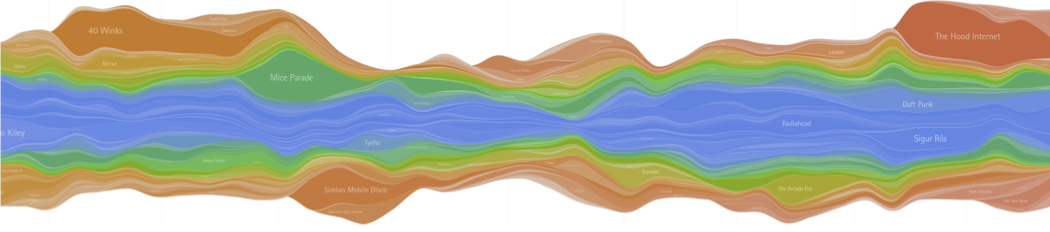
\includegraphics[width=13cm]{stream-graph}
  \caption{Esimerkki virtauskaaviosta \cite{byron-wattenberg:stacked-graphs}.}
  \label{fig:stream-graph}
\end{figure}

Työssä käytetyn kaavion X-akseli edustaa keskustelun yhteydessä puheenvuoroja. Y-akselille on koottu koko keskustelun puheenvuorojen asiasanat. Y-akselilla kulkevan tason paksuus osoittaa asiasanan painoarvon kyseisessä puheenvuorossa. Jos sanaa ei esiinny puheenvuorossa, kyseistä sanaa esittävä virta kapenee olemattomaksi.

\section{Chernoffin naamat}
Eräs todella tärkeä osa kommunikaatiota on ilmaisun tyyli: äänensävy, sanojen laji, eleet ja niin edelleen. Keskustelun tulkitsemisessa tällä on iso rooli. Jos keskustelu vaikka muuttuu dramaattisesti, puhetyylistä voidaan saada osviittaa mahdollisesta syystä. Ilmaisuille on tehty oma semanttinen kielensä, [ETSI TÄHÄN LIITTYVÄ SIVUSTO (Olli tietää)].

Tämä kuitenkin vaatisi litteroinnin lisäksi uudeksi työvaiheeksi puheenvuoron osien ilmaisutyylin manuaalisen analysoimisen, joka tekee tarvittavan materiaalin tuottamisesta liian työlästä. Siksi haluttiin vaihtoehtosesti kokeilla, voiko yksinkertaisilla mekanismeilla saada käsitystä keskustelun kokonaissävystä. Pyrittiin vastaamaan seuraaviin kysymyksiin:
\begin{itemize}
\item{Onko keskustelun yleinen linja myönteinen vai kielteinen?}
\item{Kuinka kypsää keskustelussa käytetty kieli on (kiroillaanko, käytetäänkö kohteliaisuutta ilmaisevia sanoja)?}
\end{itemize}

Edellämainittujen piirteiden arvoiminen koneellisesti on hankalaa puheen monimuotoisuuden ja tulkinnanvaraisuuden seurauksena. Kyseisten piirteiden ilmentämisen kokeilemiseen valittiin sanastoon perustuva laskenta. Rakennettiin sanastot, jotka sisältävät positiivisuutta ja negatiivisuutta ilmaisevia suomenkielen sanoja (liite 1), sekä kohteliaisuutta ja epäkohteliaisuutta ilmaisevia sanoja (liite 2).

Keskustelusta poimitaan kaikki sanat, jotka perusmuotoistetaan Jujun avulla. Tämän jälkeen voidaan hyödyntää kaavaa asd. Kaavalla saadaan Chernoffin naamojen piirtämiseen soveltuva lukuarvo väliltä -1 ja 1.

\begin{math}
  C(X, P, N) = \left\{ 
  \begin{array}{l l}
	\frac{| X \bigcap P | - | X \bigcap N |}{| X \bigcap P | + | X \bigcap N |} & \quad \text{$jos$ } {| X \bigcap P | + | X \bigcap N | > 0},\\
	0 & \quad \text{$jos$ } {| X \bigcap P | + | X \bigcap N |} = 0.\\	
  \end{array} \right.
\end{math}

Kaavassa X edustaa keskustelun sanajoukkoa. P ja N ovat sanastoja. P on joukko, joka sisältää sanat, jotka täsmätessään X:n sanajoukon kanssa tekee lukuarvosta suuremman. N-joukko taas toimii vastakkaisesti.

Ratkaisuksi valikoitui Chernoffin naamat. Kyseisellä visualisointimenetelmällä pyrittiin luomaan keskustelun ilmapiiristä ihmiselle nopeasti hahmotettava kuva. Chernoffin naamoissa on 18 erilaista kasvonpiirteen mallia, joihin kuuluu esimerkiksi seuraavat:
\begin{itemize}
\item{pään muoto}
\item{nenän pituus}
\item{silmien koko ja vinous}
\item{silmien epäkeskisyys ja erillisyys}
\item{kulmakarvat ja katseen suunta}
\item{suun kaarevuus, leveys ja korkeus.}
\end{itemize}

\begin{figure}[H]
  \centering
  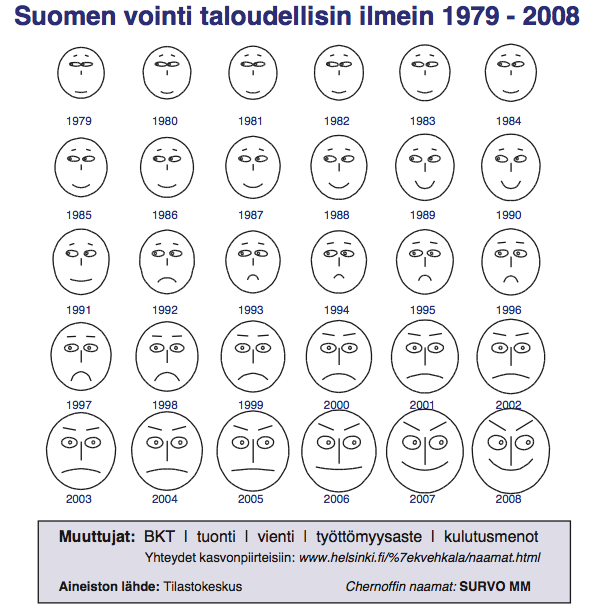
\includegraphics[width=8cm]{suomen-vointi-chernoff}
  \caption{Esimerkki Chernoffin naamoista: Suomen vointi taloudellisin ilmein \cite{helsinki:chernoffin-naamat}.}
  \label{fig:suomen-vointi-chernoff}
\end{figure}

\section{Pelilliset elementit}
Gamificationin perusidea on se, että pyritään tuomaan esimerkiksi videopeleistä tuttuja elementtejä arkipäivän rutiineihin. Usein tarkoituksena on motivoida työntekijää suoriutumaan tehtävistään.

Yksi pelielementtien piirteistä ovat "saavutukset", joita yleensä visualisoidaan kunniamerkkejä muistuttavilla grafiikoilla. Työn yhteydessä tätä sovelletaan korostamalla keskustelun osallisia. Erilaisia keskustelijoita ja heidän piirteitään nostetaan esiin esimerkiksi seuraavilla kriteereillä:
\begin{itemize}
\item{eniten sanoja}
\item{vähiten sanoja}
\item{eniten puheenvuoroja.}
\end{itemize}

\begin{figure}[H]
  \centering
  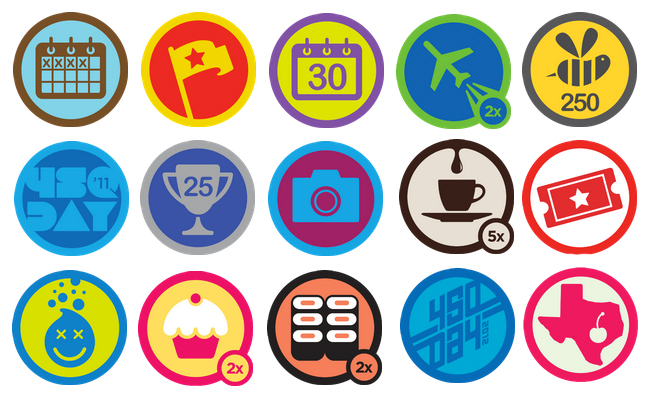
\includegraphics[width=7cm]{foursquare-kunniamerkit}
  \caption{Erilaisia merkkejä saavutusten osoittamiseksi (Foursquare-palvelussa).}
  \label{fig:foursquare-merkit}
\end{figure}

Pelielementtien käytössä on mahdolliset haittapuolensa. Jos mekanismille annetaan liikaa painoarvoa, keskustelun osalliset saattavat keskittyä tavoittelemaan edellämainittuja korostuksia, jotka voidaan luontaa palkinnonomaisiksi kannusteiksi. Ulkoinen motivaation lähde saattaa ohjata pois laadukkaasta keskustelusta \cite{jiang:dangers-of-gamification}. Mahdollisten riskien takia korostukset pyrittiin pitämään mahdollisimman neutraaleina, ja välttää palkintomuotoja.

\chapter{Tulosten todentaminen ja jatkokehitys}
Tällä hetkellä sovellus pyrkii olemaan kohtuullisen yleispätevä erikoistumatta mihinkään tiettyyn keskusteluvariaatioon. Jatkossa ohjelmistoa voisi jatkokehittää erikoistumaan erilaisiin sovellutuksiin. Eräs idea olisi hahmottaa yksittäisten henkilöiden välisten suhteiden lisäksi vuorovaikutusta isommassa mittakaavassa. Tämä voitaisiin saavuttaa erilaisten tunnisteiden lisäämisellä käsiteltävään materiaaliin. Yksi vaihtoehto olisi, että henkilölle määriteltäisiin ryhmä, johon hän kuuluu. Näin voitaisiin esimerkiksi politiikan viitekehyksessä havaita, miten puolueiden ajamat aihepiirit eroavat toisistaan.

Analysoinnin reaaliaikaisuus tekisi sovelluksesta käyttökelpoisen esimerkiksi palaverien yhteydessä, jolloin sen avustuksella voisi ohjata palaverien kulkua. 

Jos tulevaisuudessa automaattinen reaaliaikainen litterointi tulisi käyttökelpoiseksi, voitaisiin analysointikin reaaliaikaistaa. 

Jotta päästäisiin tarkempaan lopputulokseen sisällön analysoinnin suhteen, sovelluksen pitäisi olla tietoinen kontekstista. Esimerkiksi kansanedustajien täysistuntoja tarkkailtaessa esiin nousee tilanteen vaatimaan protokollaan liittyviä asiasanoja, kuten puhemies, joka on käsiteltävän asian kannalta täysin epäolennainen. 

Alkuperäisessä visiossa pyrittiin käsittelemään keskustelua hyvinkin tarkalla tasolla, ottaen huomioon enemmän yksittäisten puheenvuorojen sisältöä. Joustavuuden nimissä haluttiin laajentaa skooppia ... ja keskittyä enemmänkin keskustelun etenemisen seuraamiseen isommassa mittakaavassa.

Jatkokehityksen kannalta olisi tärkeää visualisointien tulkintojen todentaminen.

Todennettiin subjektiivisesti, että Juju tuottaa tarpeeksi pätevää asiasanoitusta myös keskustelujen osalta.

%----------------------------------------------------------------------------------------
%   BIBLIOGRAPHY 
%----------------------------------------------------------------------------------------

\bibliographystyle{vancouver}
%line space
\singlespacing
\begin{flushleft}
  \bibliography{biblio}
\end{flushleft}

\end{document}